\chapter{Generazione dei Segnali Principali}

%--------------------------------------------------------------------------------------------

Per la realizzazione del segnale a rampa e a triangolo si decide di procedere in ogni caso
per via digitale, utilizzando dei contatori binari abbinati ad un convertitore
digitale-analogico.
\medskip

\begin{figure}[ht]
    \centering
    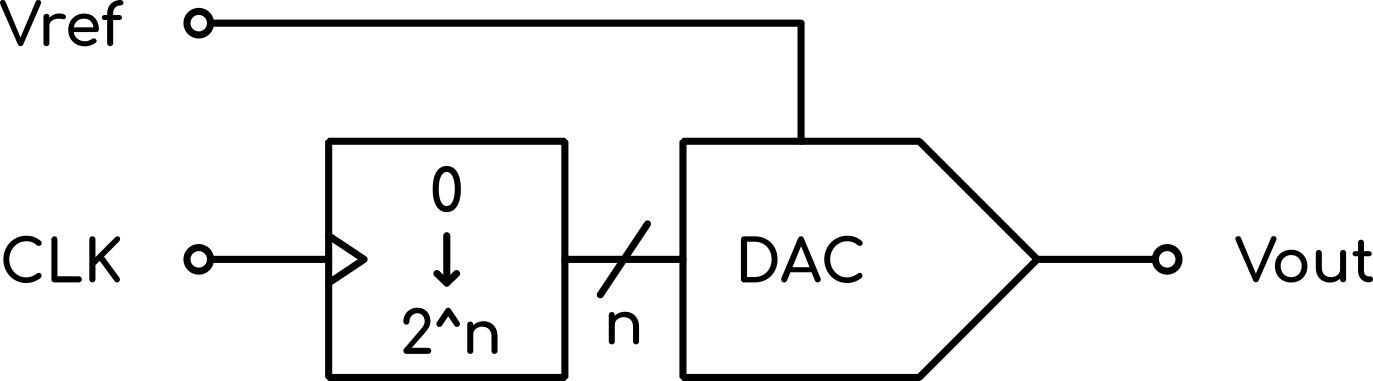
\includegraphics{block_diagrams/counter_block_diagram.png}
    \caption{Schema a blocchigenerale di un generatore di segnale}
    \label{counter_block_diagram}
\end{figure}

%--------------------------------------------------------------------------------------------

\section{Rampa}

%--------------------------------------------------------------------------------------------

\subsection*{Principio di Funzionamento}

%--------------------------------------------------------------------------------------------

Per la generazione del segnale a rampa, si fa uso di un contatore unidirezionale, ovvero in
grado di contare automaticamente da $0$ a $2^n$, dove $n$ corrisponde al numero di bit,
semplicemente fornendo un segnale di clock adeguatamente dimensionato. Maggiore il numero di
bit $n$, maggiore sarà la precisione del nostro segnale e quindi minore l'intensità del rumore
generato.
\medskip

\begin{figure}[ht]
    \centering

    \begin{subfigure}{.5\textwidth}
        \centering
        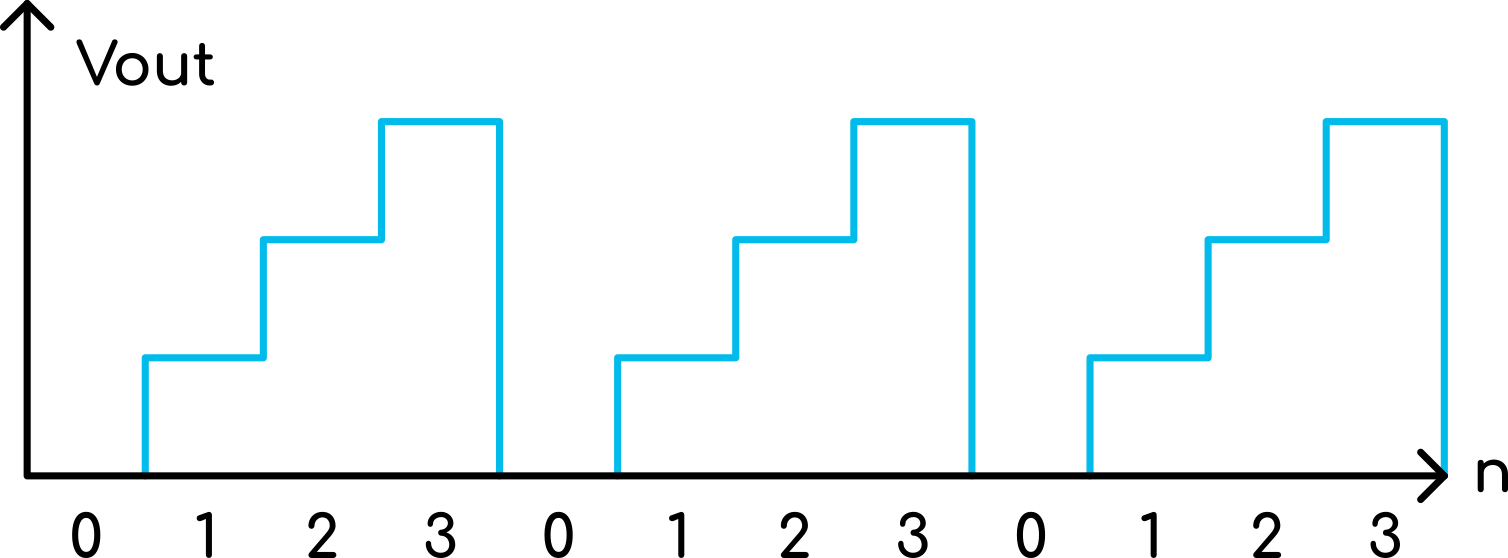
\includegraphics{graphs/low_res_ramp.png}
        \caption{Rampa ottenuta utilizzando 2 bit}
        \label{low_res_ramp}
    \end{subfigure}%
    \begin{subfigure}{.5\textwidth}
        \centering
        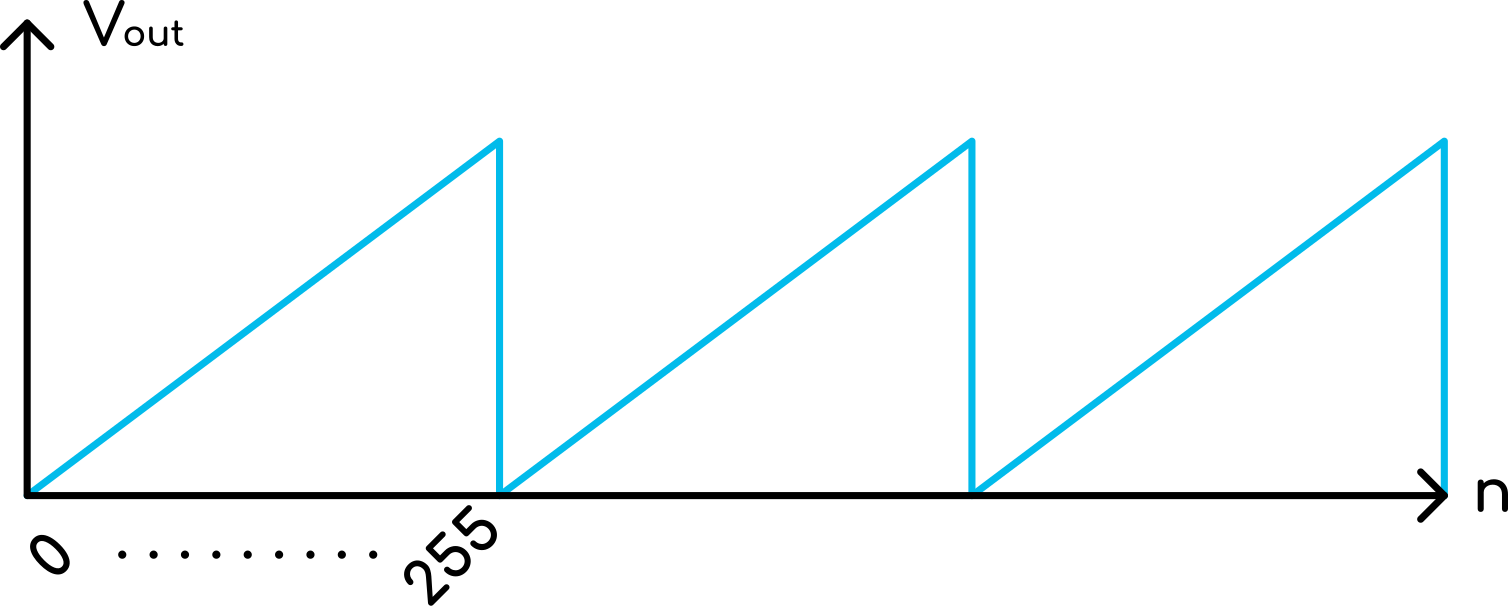
\includegraphics{graphs/high_res_ramp.png}
        \caption{Rampa ottenuta utilizzando 8 bit}
        \label{high_res_ramp}
    \end{subfigure}

    \caption{Confronto tra contatori unidirezionali con diverso numero di bit}
    \label{ramps}
\end{figure}

Tuttavia aumentando il numero di bit del contatore, è facile intuire che, a parità di
frequenza del segnale in uscita, la frequenza del segnale di clock debba necessariamente
aumentare.

Vale quindi la seguente relazione:

$$f_{signal}=\frac{f_{clk}}{2^n}$$

poichè il contatore deve effettuare un conteggio completo in un periodo del segnale in uscita.
Questo implica un limite massimo al numero di bit del contatore.

Un valore ottimale per il numero di bit è $8$, valore che ci consente infatti di limitare
al $MHz$ la frequenza do clock, contare fino a $255$ e dividere l'intervallo di tensione
d'uscita in altrettanti livelli, ottenendo quindi una variazione di

$$V_{step}=\frac{2V_{ref}}{2^n}=\frac{10V}{256}\approx39mV$$

per ogni singolo bit (scegliendo $V_{ref}=+5V$).

Lo schema a blocchi diventa quindi il seguente:
\medskip

\begin{figure}[ht]
    \centering
    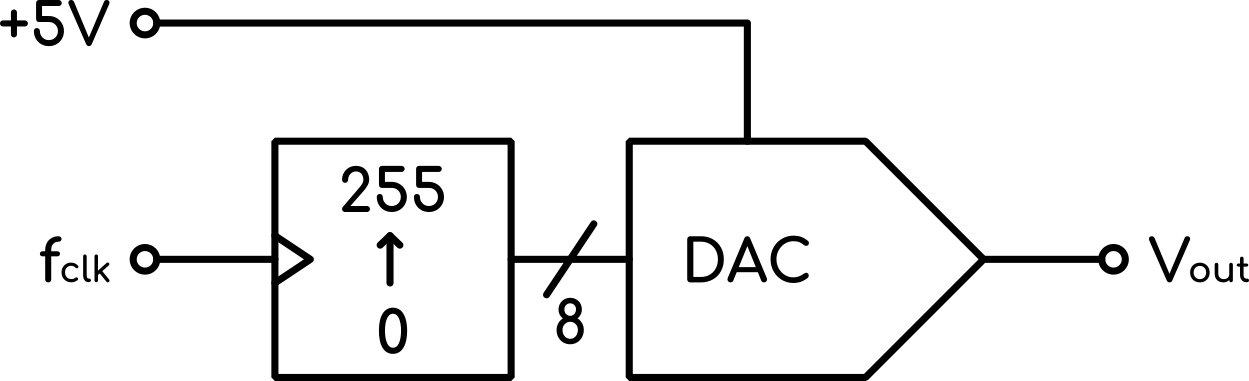
\includegraphics{block_diagrams/ramp_block_diagram.png}
    \caption{Schema a blocchi del sottosistema per la generazione della rampa}
    \label{ramp_block_diagram}
\end{figure}

A questo punto possiamo calcolare le frequenze del segnale di clock da generare,
andando a vedere quali sono le frequenze desiderate:

\begin{itemize}
    \item Valore minimo (nota A0): $f_{signal-min}=27.5Hz\rightarrow f_{clk-min}\approx7kHz$
          a cui corrisponderà un ingresso di $0V$;
    \item Valore massimo (nota A8): $f_{signal-max}\approx7kHz\rightarrow f_{clk-max}\approx1.8MHz$
          a cui corrisponderà un ingresso di $8V$;
\end{itemize}

estendendo quindi il range di funzionamento lungo 8 ottave.

%--------------------------------------------------------------------------------------------

\subsection*{Componenti Utilizzati e Schemi Elettrici}

%--------------------------------------------------------------------------------------------

Si passa ora alla scelta dei componenti per la realizzazione del blocco circuitale.

\begin{itemize}
    \item Contatore: 74HC590 \cite{74hc590};
    \item DAC: DAC0800 \cite{dac0800};
\end{itemize}

Per il circuito DAC si utilizza lo schema a pg.10 del relativo datasheet del componente.
Tale configurazione ci permette infatti di convertire il dato binario in un valore compreso
nell'intervallo $\pm V_{ref}= \pm 5V$ e $-V_{ref}= -5V$, tuttavia si utilizzano un amplificatore
operazionale e dei resistori di valore differente (rispettivamente TL074 \cite{tl074} e
$R_L=\bar{R_L}=R_{ref}=3.3k\Omega$). Si noti che anche $V_{ref}$ viene scelta diversa rispetto
allo schema nel datasheet ($+5V$), in modo da garantire le specifiche di progetto sul segnale
in uscita.
\medskip

\begin{figure}[ht]
    \centering
    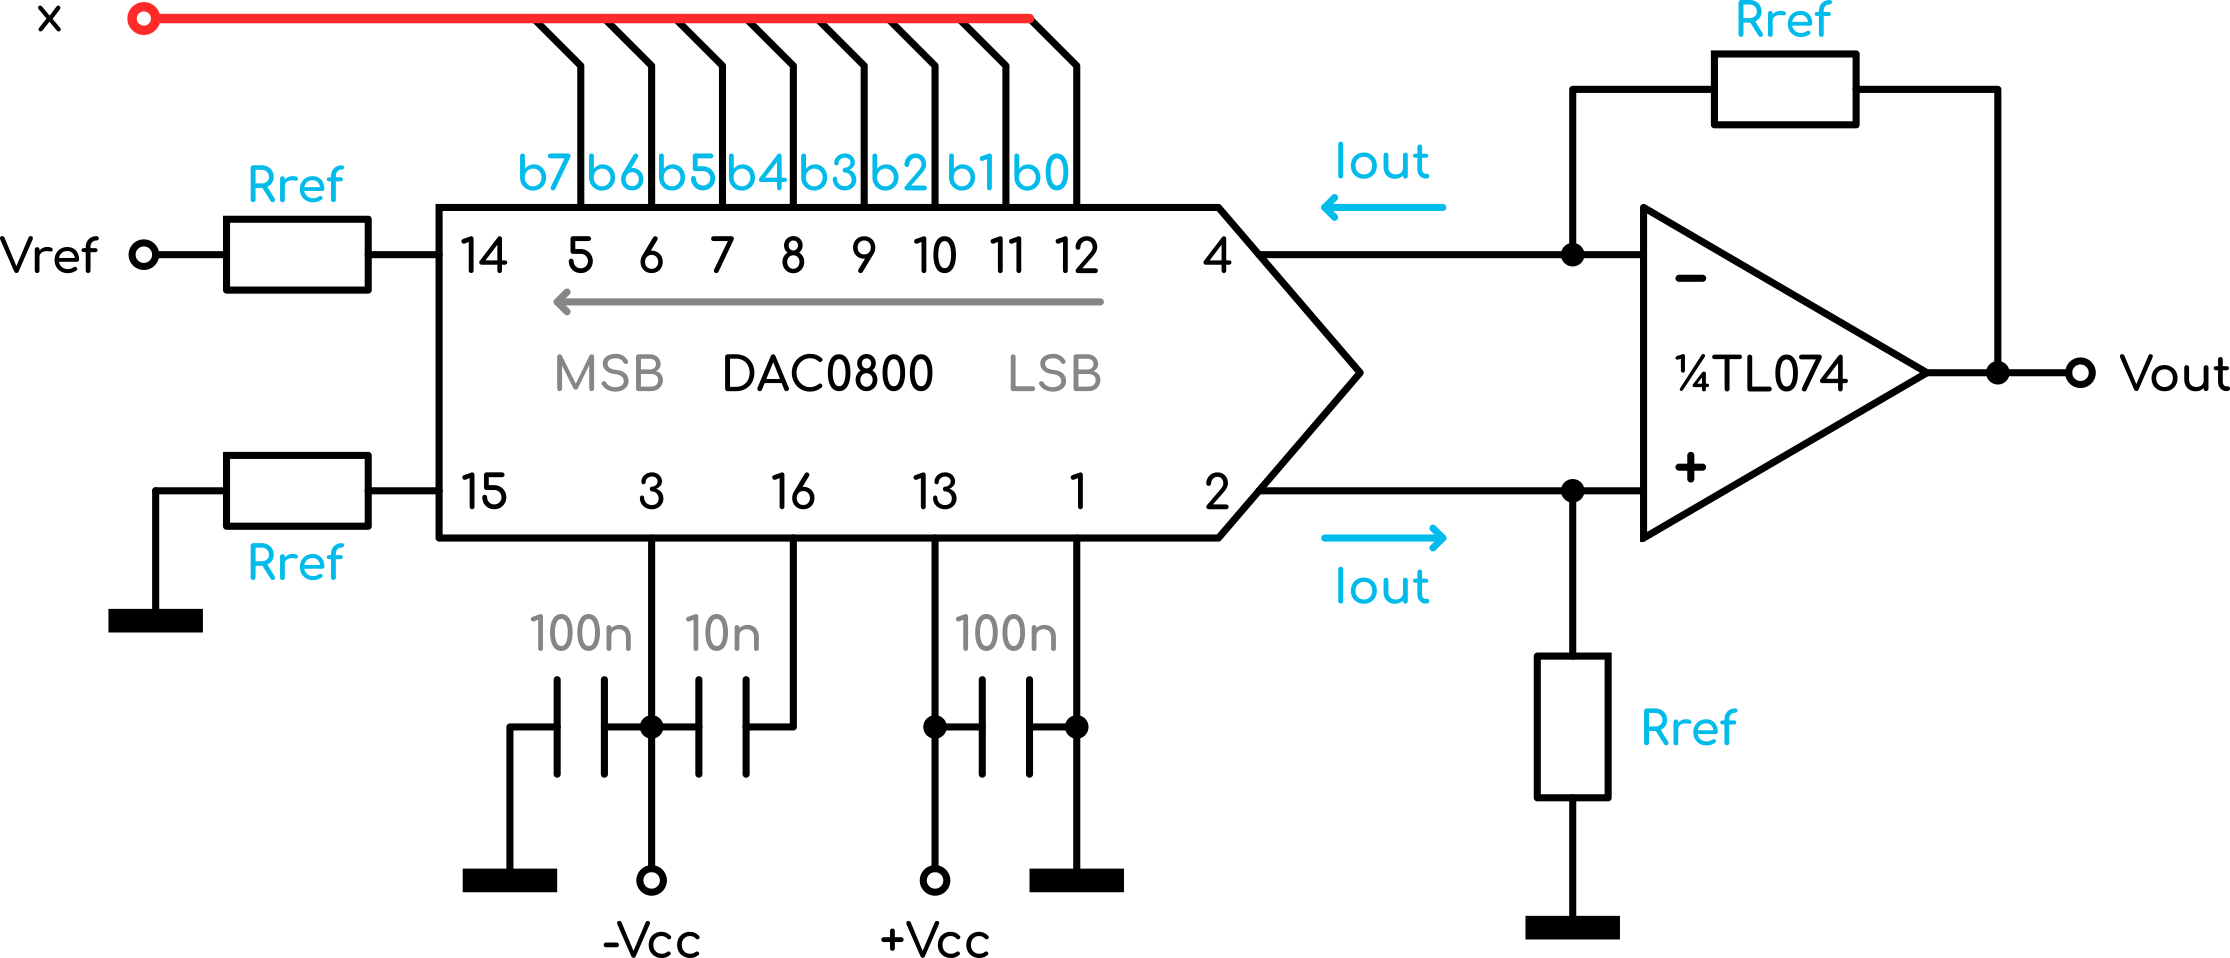
\includegraphics{circuits/DAC_circuit.png}
    \caption{Schema elettrico del DAC, $\pm V_{cc}=\pm 12V$}
    \label{DAC_circuit}
\end{figure}

Il DAC eroga una corrente $I_{out}$ proporzionale all'ingresso binario $x$, la quale viene poi
convertita in una tensione con un operazionale, in questo modo la tensione d'uscita sarà
legata al valore digitale in ingresso secondo la seguente relazione:

$$V_{out}=V_{ref}\left(\frac{2x-255}{256}\right)=5\left(\frac{2x-255}{256}\right)[V]$$

Il contatore invece viene collegato nel seguente modo:
\medskip

\begin{figure}[ht]
    \centering
    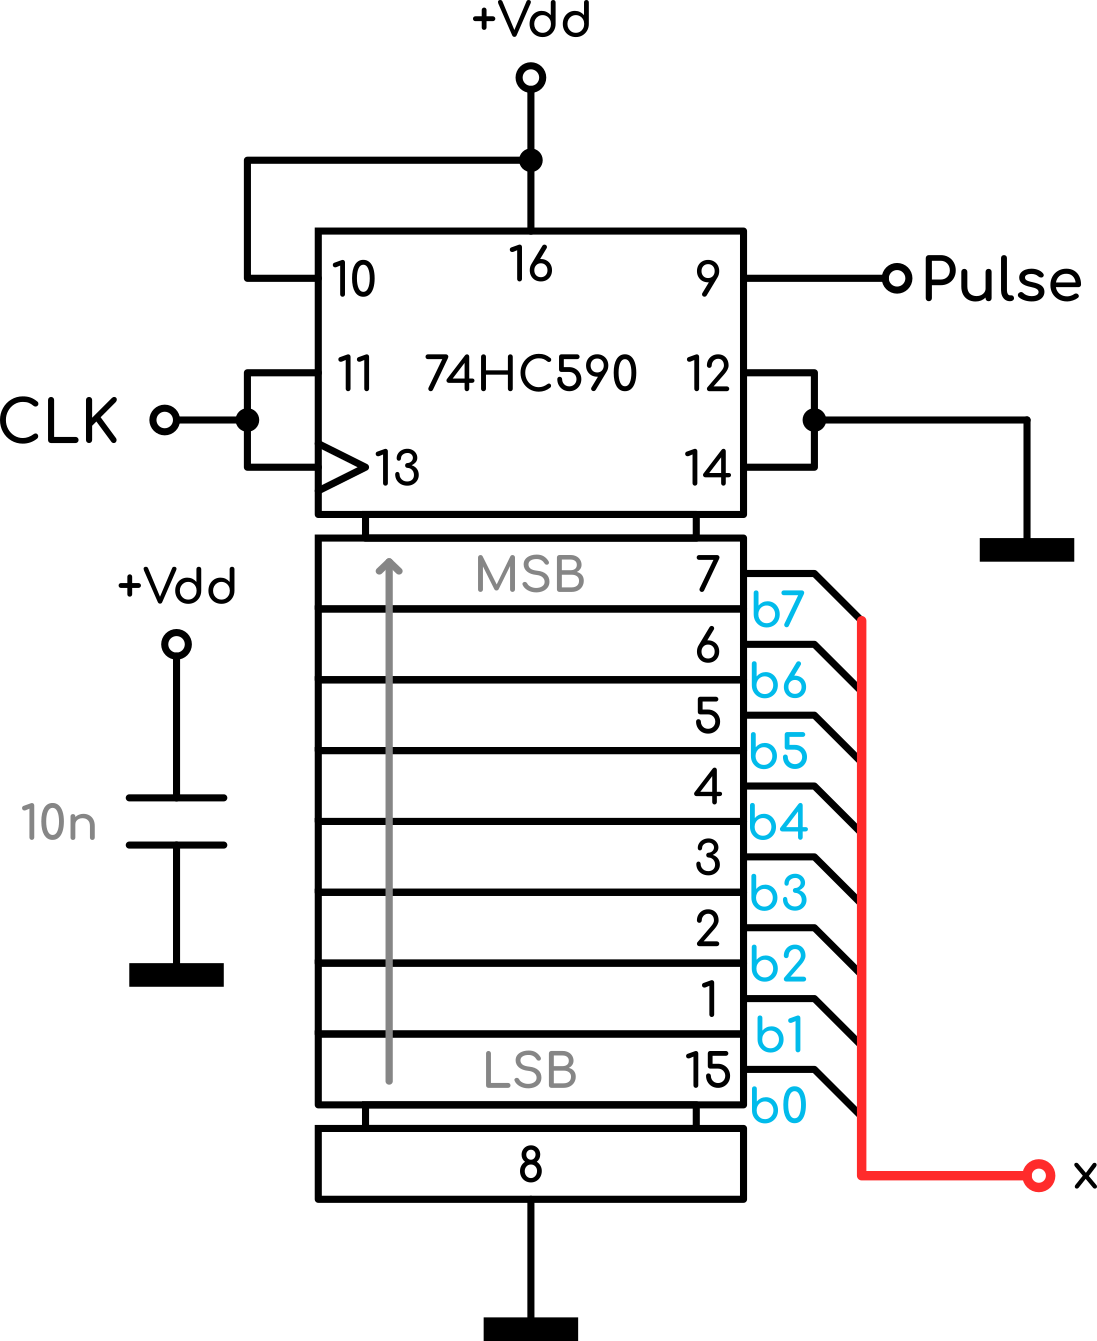
\includegraphics{circuits/ramp_counter_circuit.png}
    \caption{Schema elettrico del contatore per l'onda a rampa, $V_{dd}=+5V$}
    \label{ramp_counter_circuit}
\end{figure}

Si noti l'uscita "Pulse" in figura \ref{ramp_counter_circuit} dalla quale viene prelevato
il segnale a impulso precedentemente accennato, di cui si parlerà più in dettaglio nei
successivi capitoli.

Collegando i due blocchi insieme quindi, l'andamento della tensione $V_{out}$ sarà simile a
quello rappresentato in figura \ref{high_res_ramp} e ad ogni impulso di clock corrisponderà
un gradino di tensione di circa $40mV$ come calcolato precendentemente.

%--------------------------------------------------------------------------------------------

\subsection*{Risultati Pratici}

\begin{figure}[ht]
    \centering

    \begin{subfigure}{.5\textwidth}
        \centering
        
\includegraphics{misc/oscilloscope_placeholder.png}
        \caption{Acquisizione del segnale a rampa reale}
        \label{acq_ramp}
    \end{subfigure}%
    \begin{subfigure}{.5\textwidth}
        \centering
        
\includegraphics{misc/oscilloscope_placeholder.png}
        \caption{Zoom degli step della rampa acquisita + clock}
        \label{acq_ramp_steps}
    \end{subfigure}

    \caption{Acquisizioni del segnale a rampa}
    \label{acq_ramp_signals}
\end{figure}

%--------------------------------------------------------------------------------------------

\section{Triangolo}

%--------------------------------------------------------------------------------------------

\subsection*{Principio di Funzionamento}

%--------------------------------------------------------------------------------------------

Il principio di funzionamento è del tutto analogo a quello del contatore per il segnale a
rampa, tuttavia in questo caso, il contatore utilizzato è bidirezionale e necessita di un
segnale che determini la direzione di conteggio (up o down).
\medskip

\begin{figure}[ht]
    \centering
    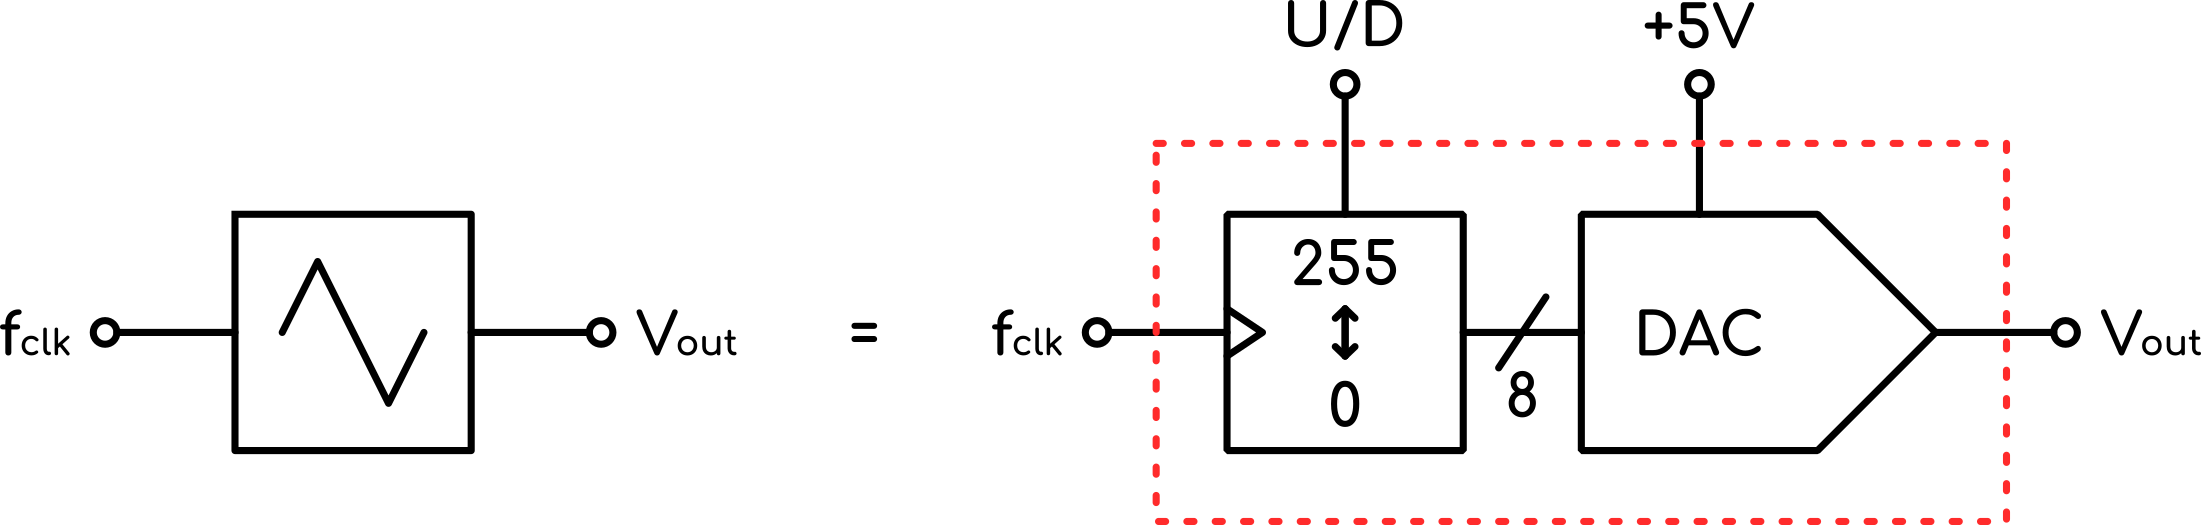
\includegraphics{block_diagrams/triangle_block_diagram.png}
    \caption{Schema a blocchi del sottosistema per la generazione del triangolo}
    \label{triangle_block_diagram}
\end{figure}

\begin{figure}[ht]
    \centering

    \begin{subfigure}{.5\textwidth}
        \centering
        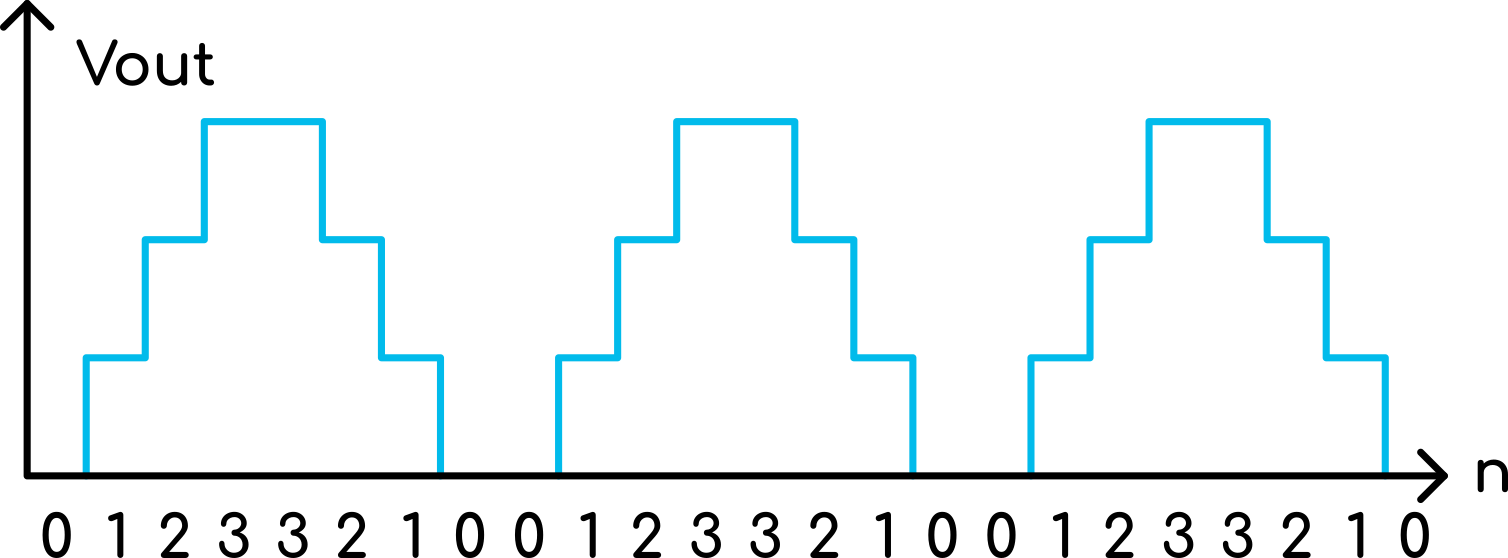
\includegraphics{graphs/low_res_triangle.png}
        \caption{Triangolo ottenuto utilizzando 2 bit}
        \label{low_res_triangle}
    \end{subfigure}%
    \begin{subfigure}{.5\textwidth}
        \centering
        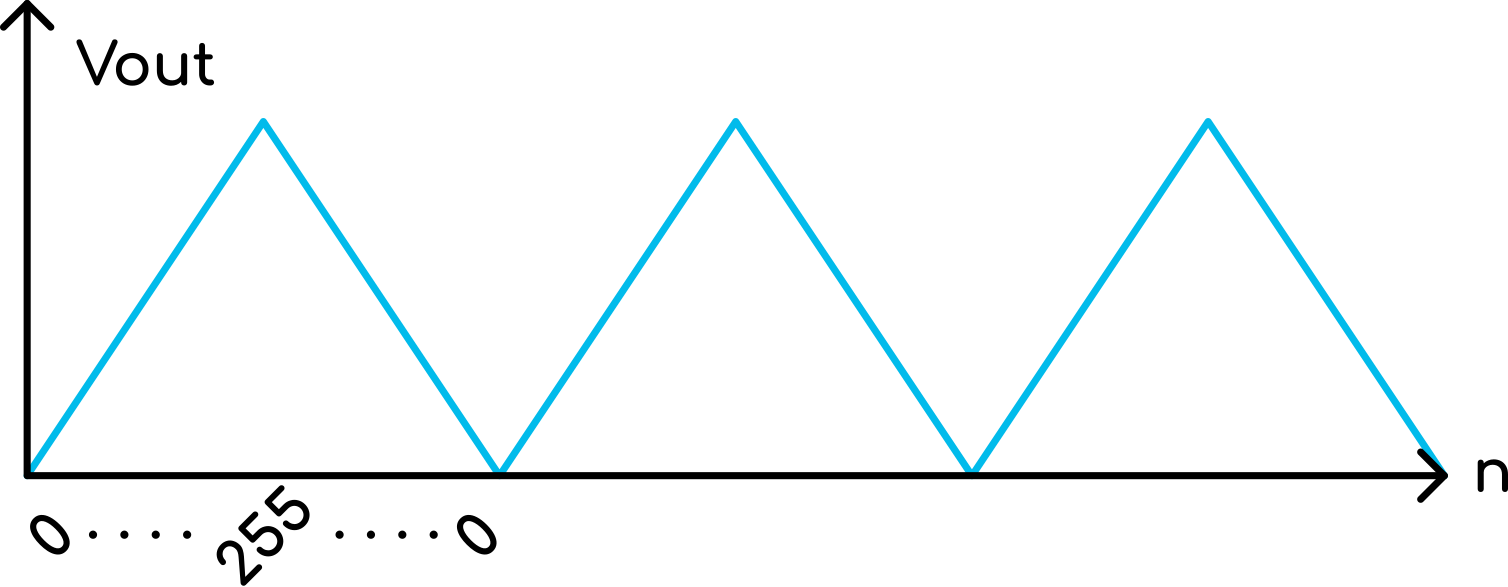
\includegraphics{graphs/high_res_triangle.png}
        \caption{Triangolo ottenuto utilizzando 8 bit}
        \label{high_res_triangle}
    \end{subfigure}

    \caption{Confronto tra contatori bidirezionali con diverso numero di bit}
    \label{triangles}
\end{figure}

Anche la configurazione del DAC rimane quella rappresentata in figura \ref{DAC_circuit},
utilizzata per la rampa.

Va tuttavia fatta notare una importante differenza, poichè in questo caso il numero di cicli
di clock per il conteggio è doppio rispetto a quello del contatore per la rampa. Infatti
dovranno essere eseguiti 256 conteggi verso l'alto e 256 conteggi verso il basso per effettuare
un singolo periodo di onda triangolare. Ne consegue quindi che la frequenza di clock in ingresso
a questo sottosistema dovrà essere doppia rispetto a quella della sezione per la rampa, come
risulta evidente in figura \ref{steps}.
\medskip

\begin{figure}[ht]
    \centering

    \begin{subfigure}{.5\textwidth}
        \centering
        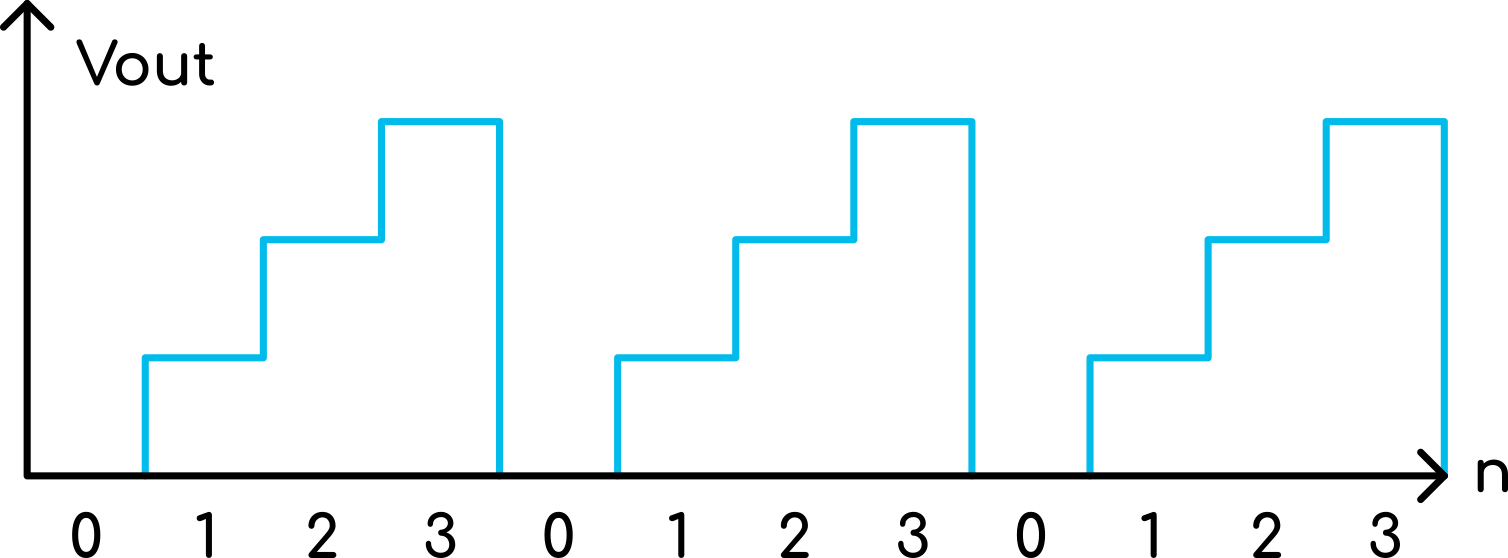
\includegraphics{graphs/low_res_ramp.png}
        \caption{Rampa ottenuta utilizzando 2 bit}
    \end{subfigure}%
    \begin{subfigure}{.5\textwidth}
        \centering
        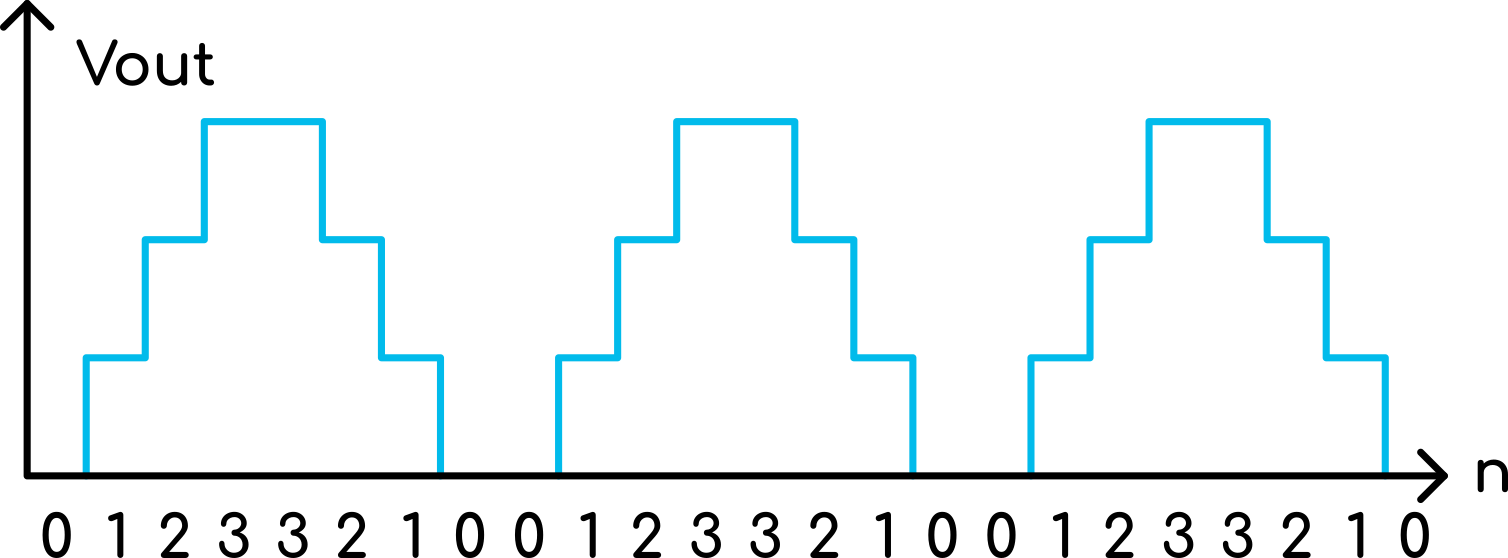
\includegraphics{graphs/low_res_triangle.png}
        \caption{Triangolo ottenuto utilizzando 2 bit}
    \end{subfigure}

    \caption{Confronto del conteggio tra contatori unidirezionali e bidirezionali}
    \label{steps}
\end{figure}

%--------------------------------------------------------------------------------------------

\subsection*{Componenti Utilizzati e Schemi Elettrici}

L'unico componente diverso rispetto al circuito per la rampa è il contatore, che come detto
deve essere bidirezionale. Si utilizzano due 74LS169 \cite{74ls169} in cascata, con la seguente
configurazione:
\medskip

\begin{figure}[ht]
    \centering
    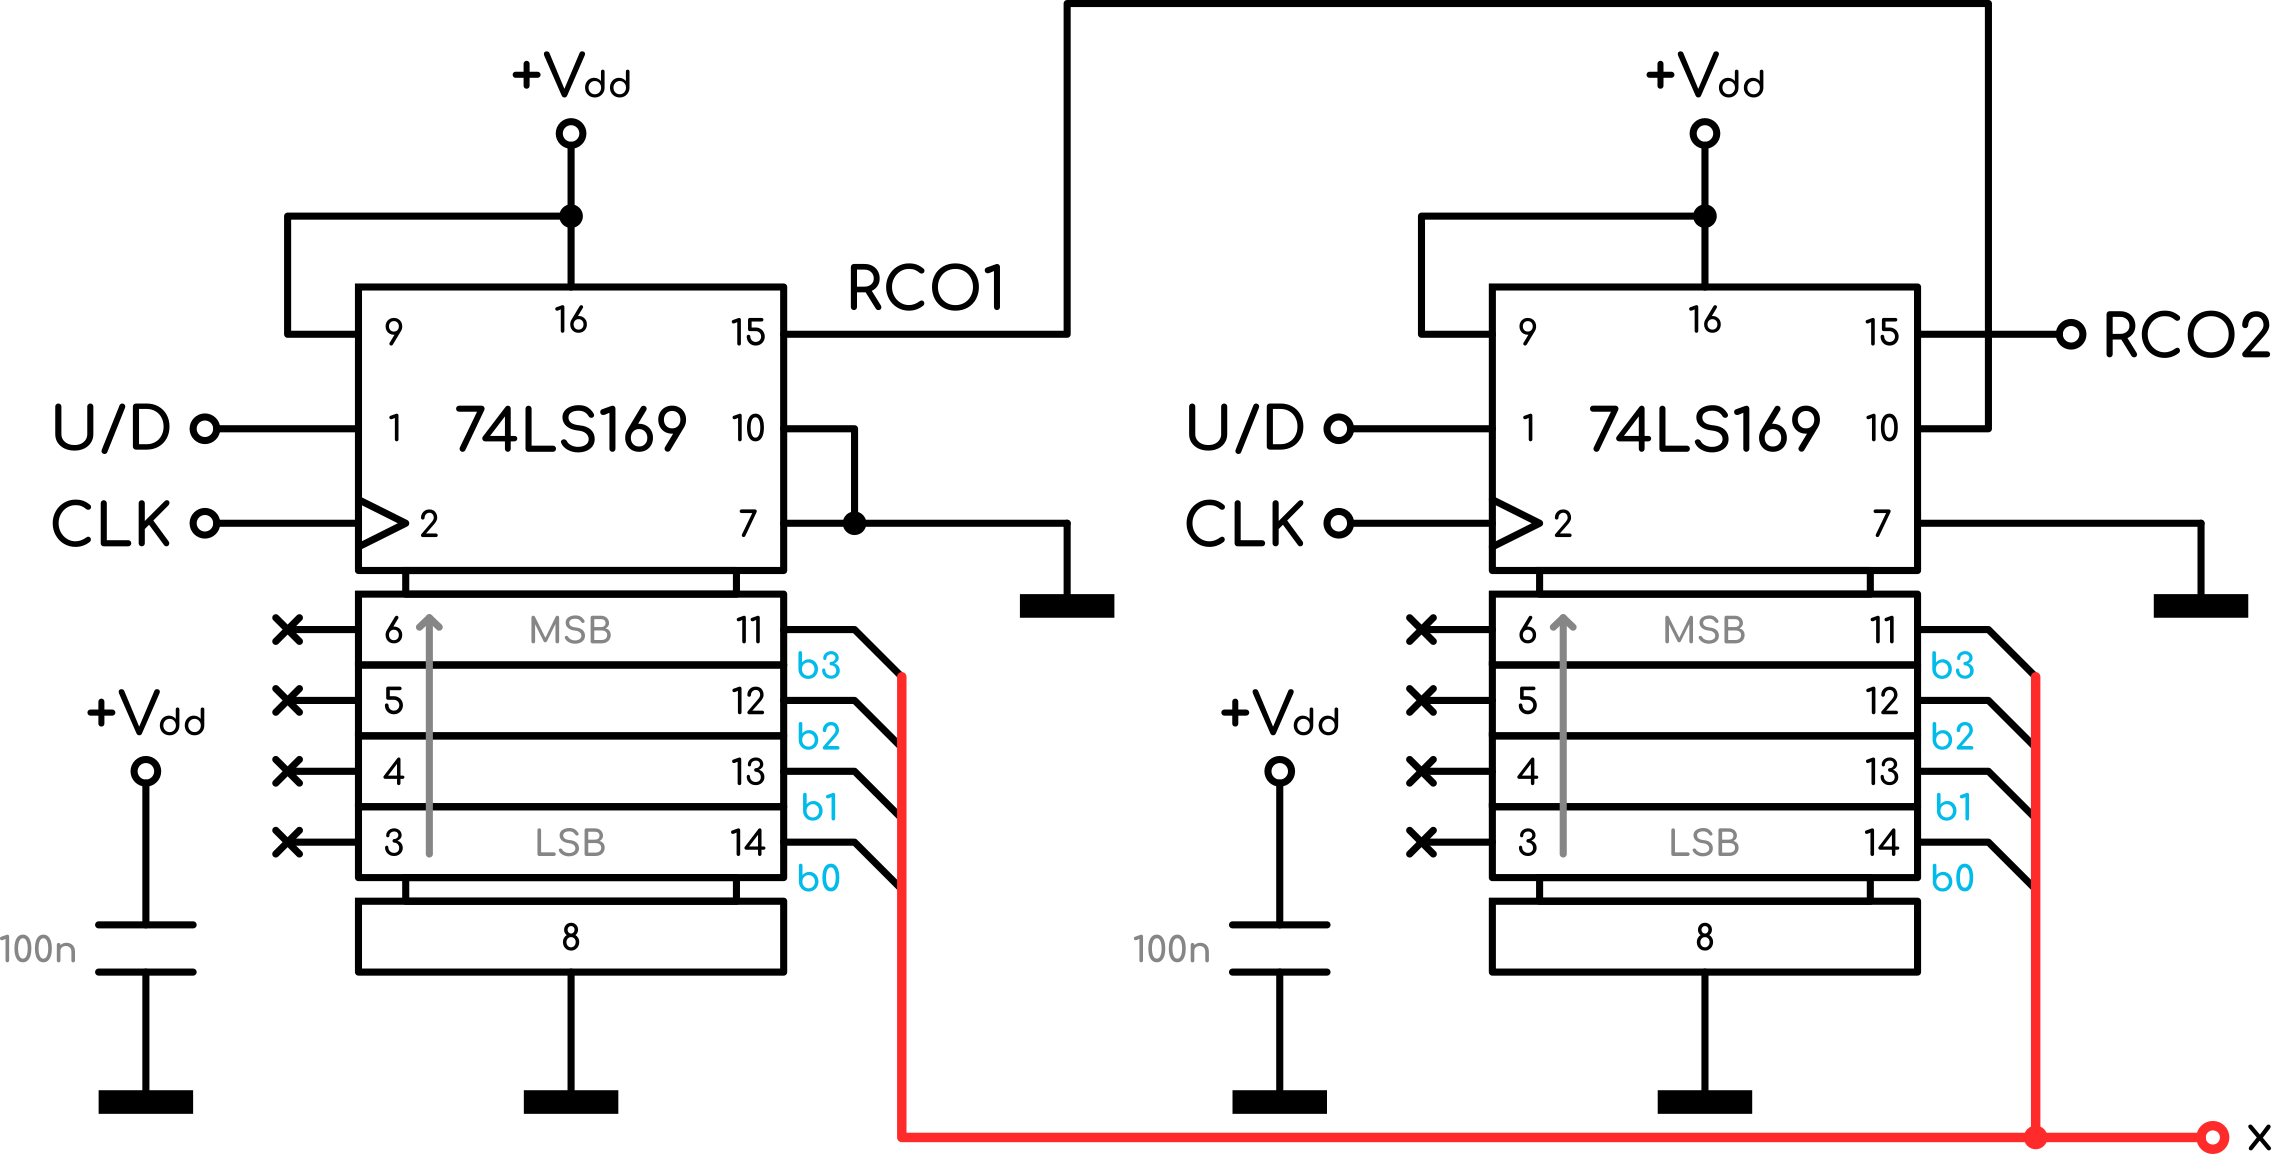
\includegraphics{circuits/triangle_counter_circuit.png}
    \caption{Schema elettrico dei contatori per l'onda triangolare, $V_{dd}=+5V$}
    \label{triangle_counter_circuit}
\end{figure}

Il componente utilizzato presenta anche degli ingressi per il preset del numero di partenza
(pin da 3 a 6), che però nel nostro caso non vengono utilizzati.

L'uscita denominata $RCO2$ verrà utilizzata per pilotare il verso del conteggio, utilizzando
una soluzione circuitale meglio descritta nella sezione successiva.

%--------------------------------------------------------------------------------------------

\subsection*{Risultati Pratici}

\begin{figure}[ht]
    \centering

    \begin{subfigure}{.5\textwidth}
        \centering
        
\includegraphics{misc/oscilloscope_placeholder.png}
        \caption{Acquisizione del segnale a triangolo reale}
        \label{acq_triangle}
    \end{subfigure}%
    \begin{subfigure}{.5\textwidth}
        \centering
        
\includegraphics{misc/oscilloscope_placeholder.png}
        \caption{Zoom degli step del triangolo acquisito + clock}
        \label{acq_triangle_steps}
    \end{subfigure}

    \caption{Acquisizioni del segnale a triangolo}
    \label{acq_triangle_signals}
\end{figure}

%--------------------------------------------------------------------------------------------

\section{Adattamento dei Segnali di Clock}

Si è visto come, per avere la stessa frequenza di segnale d'uscita, il contatore per il segnale
a triangolo deve avere una frequenza di clock doppia rispetto a quella del contatore per il
segnale a rampa. Questo problema si risolve facilmente utilizzando un divisore di frequenza,
ottenuto con un semplice toggle flip-flop (TFF).
\medskip

\begin{figure}[ht]
    \centering
    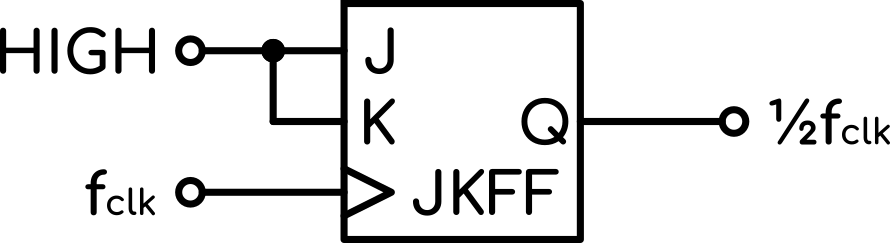
\includegraphics{block_diagrams/freq_divider_block_diagram.png}
    \caption{Schema a blocchi del divisore di frequenza}
    \label{freq_divider_block_diagram}
\end{figure}

Le specifiche sul segnale di clock ci impongono allora di generare un segnale a onda quadra
con frequenza variabile tra $\approx14kHz$ e $\approx3.6MHz$.

Invece, per fare in modo che il contatore del triangolo cambi effettivamente verso di conteggio
è necessario utilizzare un altro TFF collegato al segnale $RCO2$ invertito, poichè attivo a
livello logico basso, e all'ingresso $U/D$.
\medskip

\begin{figure}[ht]
    \centering
    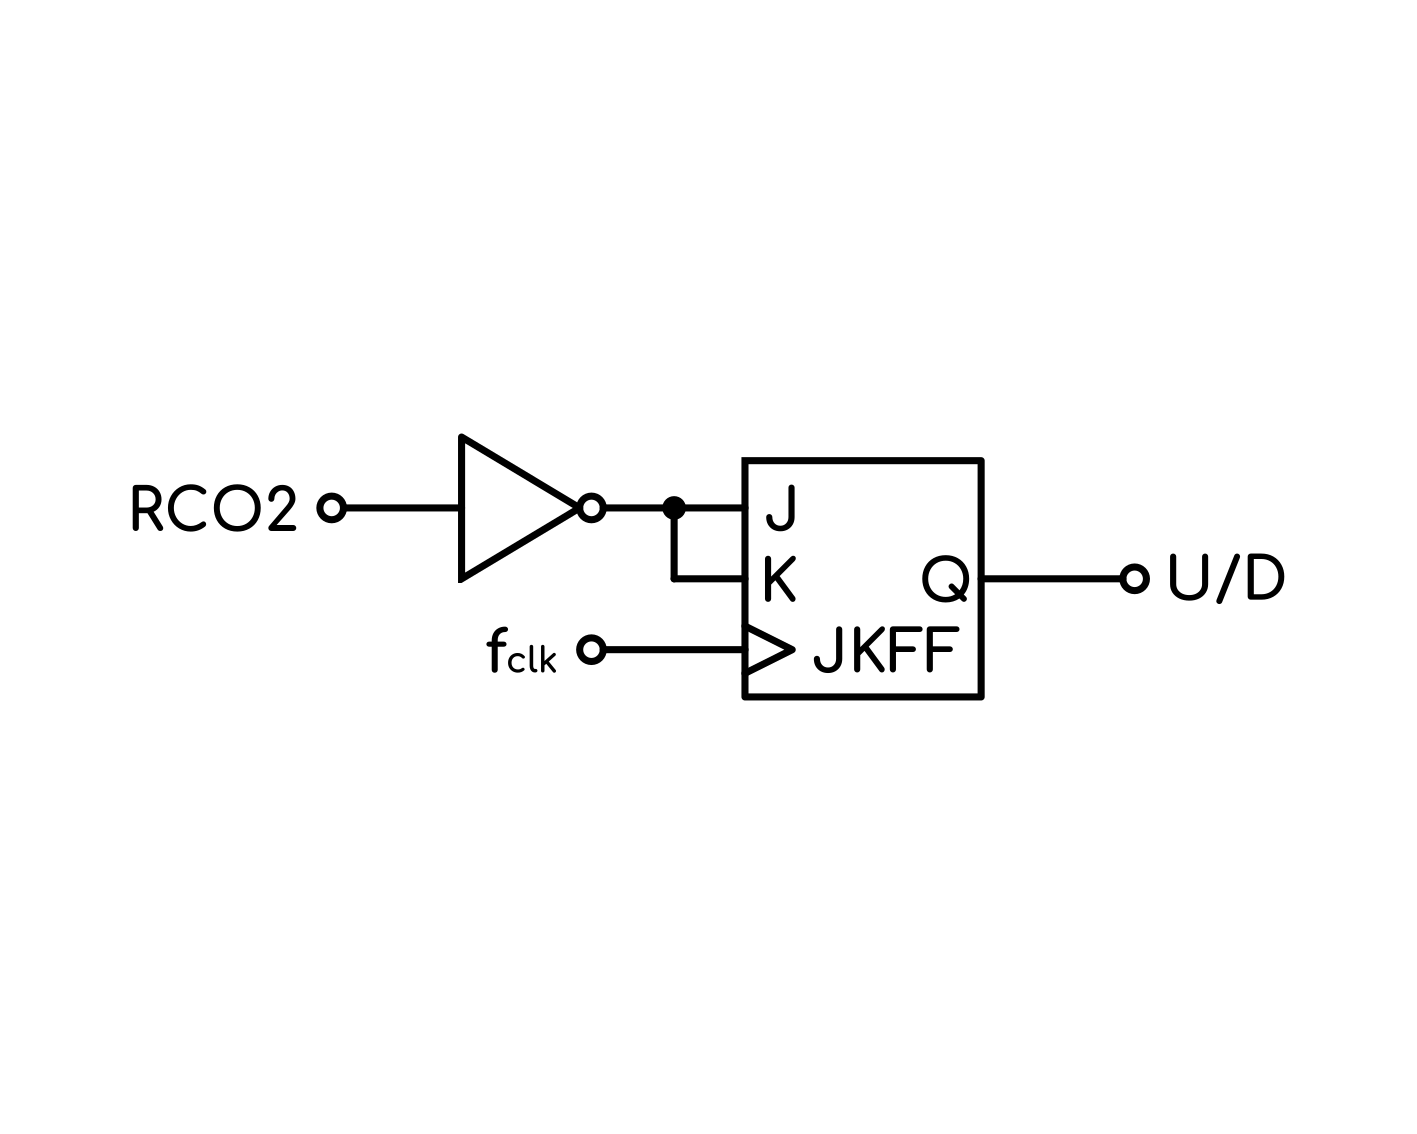
\includegraphics{block_diagrams/UD_block_diagram.png}
    \caption{Schema a blocchi del sistema per il segnale di pilotaggio}
    \label{UD_block_diagram}
\end{figure}

I componenti utilizzati per questo scopo sono:

\begin{itemize}
    \item Flip-Flop: 74HC73 \cite{74hc73};
    \item MOSFET: 2N7000 \cite{2n7000};
\end{itemize}

Il chip utilizzato per i flip-flop fornisce esattamente le 2 unità necessarie al nostro scopo.

Lo schema elettrico per l'inverter è rappresentato in figura \ref{inverter_circuit}, dove il
MOSFET utilizzato è compatibile con le tensioni logiche presenti nel circuito.
\medskip

\begin{figure}[ht]
    \centering
    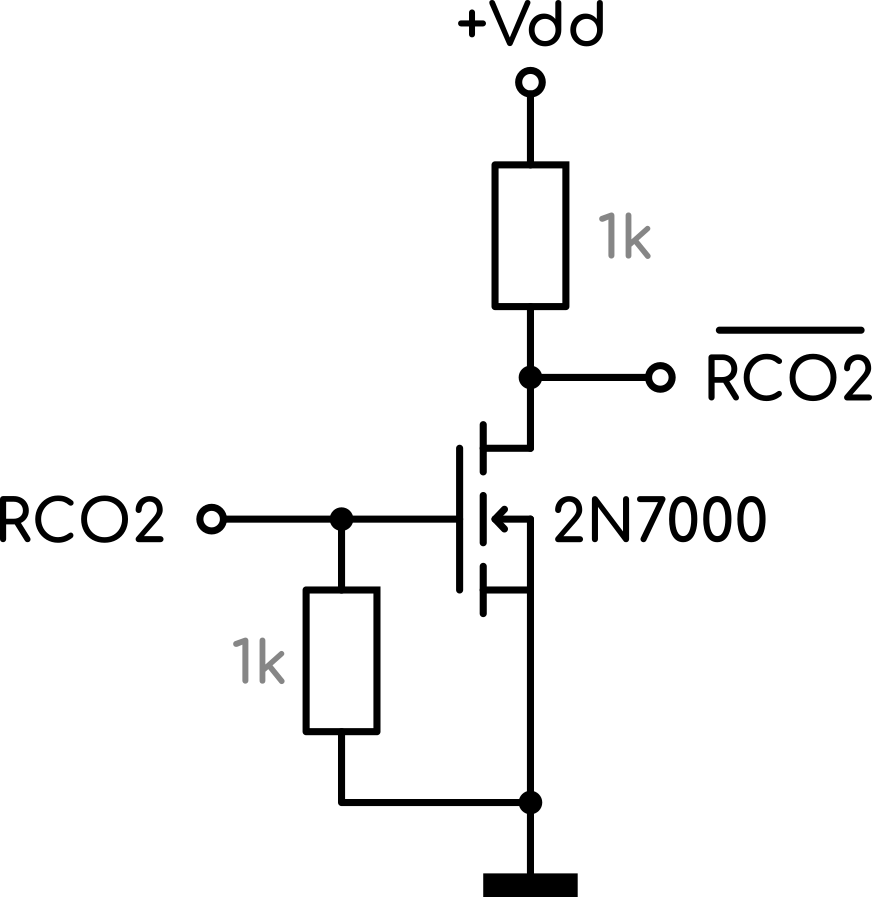
\includegraphics{circuits/inverter_circuit.png}
    \caption{Schema elettrico dell'inverter logico, $V_{dd}=+5V$}
    \label{inverter_circuit}
\end{figure}

A questo punto collegando tutti i pezzi discussi finora, otteniamo il nucleo fondamentale
del modulo,che ci permette di ottenere rampa e triangolo (e anche impulso) ad una frequenza
proporzionale a quella del segnale di clock in ingresso.
\medskip

\begin{figure}[ht]
    \centering
    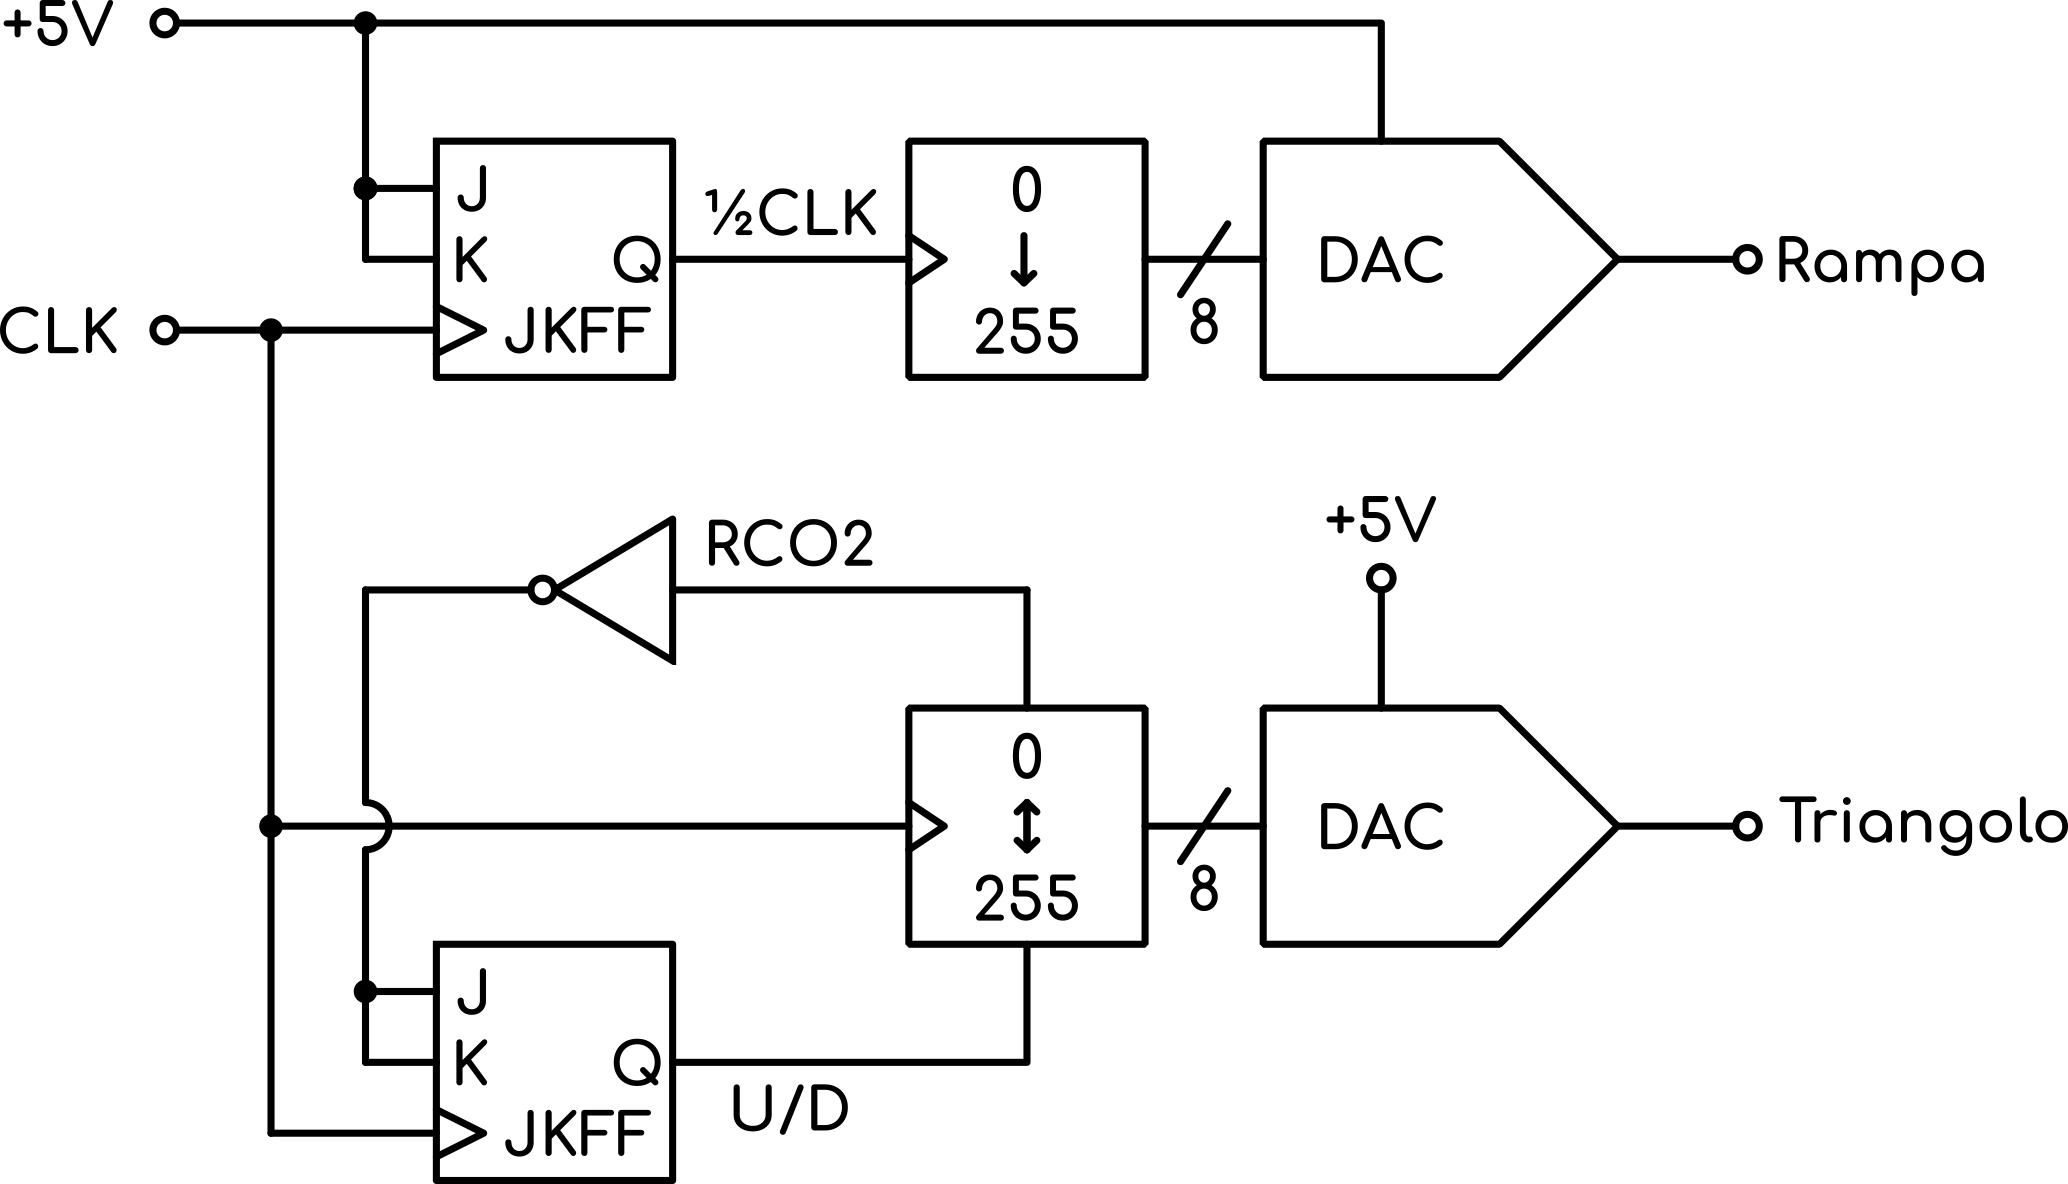
\includegraphics{block_diagrams/main_signals_block_diagam.png}
    \caption{Schema a blocchi del capitolo}
    \label{main_signals_block_diagram}
\end{figure}

%--------------------------------------------------------------------------------------------
